Sana \termi{prosentti}{prosentti} tulee latinan kielen ilmaisusta \termi{pro centum}{pro centum}, joka tarkoittaa kirjaimellisesti ''sataa kohden'' tai ''sadasta''. Prosentit ovat siis sadasosia, ja kyseessä on rationaalilukujen sovellus -- prosentteja käytetään ilmaisemaan suhteellista osuutta. Prosentit voidaan mieltää yksiköinä, jolloin käytetään prosentin symbolina \%-merkkiä. Prosentin sukulaiskäsite on \termi{promille}{promille}, joka tulee vastaavasta latinan ilmaisusta \termi{pro mille}{pro mille}. Promillen symboli on \permil.

\laatikko[Prosentti ja promille]{$1 \text{prosentti}=1\,\% = \frac{1}{100} = 0,01$\\
$1 \text{promille}=1\,\permil=\frac{1}{1\,000}=0,001$}

Erityisesti kannattaa huomata, että $100\,\%=1$. Jos prosenttiluku on annettu muodossa $p$\,\%, se voidaan aina kirjoittaa murtolukuna $\frac{p}{100}$.

\begin{esimerkki}
\alakohdat{
§ $0,03=\frac{3}{100}=3\,\%=30\,\permil$
§ $0,00478=\frac{0,478}{100}=0,478\,\%=4,78\,\permil$
§ $0,76=\frac{76}{100}=76\,\%=760\,\permil$
§ $1,23=\frac{123}{100}=123\,\%=1\,230\,\permil$
§ $2,10=\frac{210}{100}=210\,\%=2\,100\,\permil$
}
\end{esimerkki}

%Jos sadaosien lukeminen suoraan desimaaleista tuntuu haastavalta, saadaan prosentit ''näkyviin'' kertomalla desimaaliluku sadalla. Tällöin sadasosat siirtyvät luvussa ykkösten paikalle. Tämä on kuitenkin vain matemaattinen kikka vastauksen ulkoasun muuttamiseksi -- ei välttämätöntä tehtävän ratkaisun kannalta.
%
%\begin{esimerkki}
%Esittääksemme desimaaliluku $0,017$ prosentteina, luvun voi kertoa sadalla, jolloin saadaan $100\cdot 0,017=1,7$. Siis $0,017=1,7\,\%$.
%\end{esimerkki}
%suhteellinen/absoluuttinen-tarkastelu tähän vai rationaalilukujen sovelluksiin?? esimerkkinä punapaidat 25/239 ja kultapaidat 10/55! määrässä voittaa,suhteessa häviää! :) esimerkissä myös merkkaa elävien ja kuolleiden suhdetta (piirakkadiagrammi)
%
%+ näin moni EI äänestänyt... :)

Prosenttilaskennan käytännön kysymyksenasettelut ja tehtävät voidaan jakaa karkeasti neljään ryhmään. Tehtävänantojen peruskysymykset liittyvät toisiinsa seuraavalla sivulla olevan kaavion mukaisesti, missä $a$, $b$ ja $p$ sekä $x$, $y$ ja $q$ ovat (mielivaltaisia) lukuja. Vaadimme lisäksi reaalilukujen ominaisuuksiin vedoten, että $b$ ja $x$ eli luvut, joihin verrataan ovat nollasta poikkeavia. Kaavion toisessa osassa on esitetty samat kysymykset formalisoituina yhtälöiksi.
\newpage
\laatikko[Prosenttilaskennan tehtävätyypit]{
\begin{tabular}{|ccc|}
\hline 
 & & \\
\vtop{\hbox{\strut ''Kuinka monta prosenttia ($p$)}\hbox{\strut luku $a$ on $b$:stä?''}}  & $\rightleftarrows$ & \vtop{\hbox{\strut ''Kuinka paljon ($a$) on}\hbox{\strut $p$\,\% luvusta $b$?''}}\\ 
$\downarrow$ &  & $\downarrow$ \\ 
\vtop{\hbox{\strut ''Kuinka monta prosenttia ($p$)}\hbox{\strut luku $a$ on suurempi/pienempi kuin $b$?''}} & $\rightleftarrows$ & \vtop{\hbox{\strut ''Mitä ($a$) saadaan, kun $b$}\hbox{\strut kasvaa/vähenee $p$ prosenttia?''}}  \\ 
& & \\
\hline
 & & \\
\vtop{\hbox{\strut $\dfrac{a}{b}=p\,\%$}}  & $\rightleftarrows$ & \vtop{\hbox{\strut $p\,\%\cdot b=a $}}\\ 
$\downarrow$ &  & $\downarrow$ \\ 
\vtop{\hbox{\strut $\dfrac{|x-y|}{y}=q\,\%$}} & $\rightleftarrows$ & \vtop{\hbox{\strut $\left(1\pm q\,\% \right)y=x$}}\\ 
 & &\\
\hline 
\end{tabular}
}

Ongelmat, joiden välillä on nuoli molempiin suuntiin, ovat matemaattisesti yhtäläisiä eli ekvivalentteja; ne voidaan esittää ja käsitellä molemmin tavoin, vaikka ratkotaankin edelleen samaa ongelmaa. Huomaa, että yhtälöt ovat samat mutta esitetty eri muodossa.

Taulukon ylärivin kaksi tapausta ovat yksinkertaisimmat tehtävänannot, ja ne käsitellään ensin. Alarivin kysymyksenasetteluiden formalisointi (lausekkeiksi ja yhtälöksi kirjoittaminen) vaatii ylärivin kysymysten tekniikkaa. (Kaavion jäsentely tukee myös kuitenkin sitä, että ensin voitaisiin opetella vasemmalla puolella olevat ja sen jälkeen erillisesti oikealla puolella olevat tehtävätyypit -- tai toisinpäin.)

Tehtävien ratkaisu saattaa vaatia edellä mainittujen tilanteiden yhdistelemistä ja tuntemattoman ratkaisemista yhtälöstä. Erilaisten suhteiden prosentuaalisille ilmaisuille on vakiintunut omat nimensä, jotka kannattaa opetella.

\subsection{Vertailuprosentti ja perusarvo}

\laatikko[Vertailuprosentti ja perusarvo]{
    \termi{vertailuprosentti}{Vertailuprosentilla} tarkoitetaan sitä, kuinka paljon jokin on jostakin, mihin verrataan.
    Lukua, johon verrataan tai jota muutetaan, kutsutaan \termi{perusarvo}{perusarvoksi}.}

Vertailuprosentilla vastataan siis kysymykseen ''kuinka monta prosenttia luku $a$ on luvusta $b$?'', ja vertailuprosentti saadaan laskutoimituksesta $\frac{a}{b}$, joka tulkitaan lopullista vastausta varten prosentteina eli sadaosina. Koska jakolasku ei ole vaihdannainen, on tärkeää varmistaa, että tehtävässä suhde muodostetaan oikein päin. Suhdetta muodostettaessa se, mihin verrataan, toimii jakajana.

\begin{esimerkki}
Kuinka monta prosenttia
\alakohdat{
§ luku $20$ on luvusta $80$?
§ luku $80$ on luvusta $20$?
}
	\begin{esimratk}
	\alakohdat{
	§ Perusarvo on tässä tapauksessa $80$ -- siihen verrataan. Lasketaan osamäärä $\frac{20}{80}$ ja esitetään vastaus prosentteina:
	$$\frac{20}{80}=\frac{2}{8}=\frac{1}{4}=0,25=25\,\%$$
	§ Nyt perusarvo on $20$, ja siihen verrataan. Lasketaan osamäärä $\frac{80}{20}$ ja esitetään vastaus prosentteina:
	$$\frac{80}{20}=\frac{8}{2}=4=400\,\%$$
	}
	\end{esimratk}
\end{esimerkki}

%Vertailuprosentti voidaan laskea paljaiden lukujen suureista äytä, että pitää olla samaa suuretta, yksiköt kyllä supistuvat pois
%ideaaliesimerkkiketju: luvuilla -> symboleilla yleisemmin -> sanallinen sovellus
%esitä todistus, mikä yhdistää kaavion alarivin jäsenet
%esimerkkiin negatiivisia lukuja jan
%pointtina nyt se, että yhtälöt ja sitten, että voidaan käsitelläkummalla tavalla tahansa
%komplementtiesimerkki tyyliin "40 kansasta vastustaa...." -> "60 prosentita kansasta ei vastusta"
% esimerkki absoluuttisesta ja suhteellisesta kasvusta, esim- yhdsityksen jäsenmäärä ja sittnen kehuskellaan... mutta pineinllä absoluuttisilla määrillä tulee hlepomin nuo isot suhteelliset :)
% KIRKOSTAEROAMISTILASTOT!!!! -> näissä kunnissa...
% kaksi esimerkkiä liuossekoituksista, kuivauksesta yms.

\begin{esimerkki}
Tarmo leikkaa pizzan neljään osaan ja syö näistä kolme.
\alakohdat{
§ Kuinka monta prosenttia pizzasta Tarmo syö?
§ Kuinka monta prosenttia pizzasta jää jäljelle?
}
	\begin{esimratk}
\alakohdat{
§ Tarmo syö $3$ palaa neljästä eli $\frac{3}{4} = 0,75$. Tämä voidaan muuttaa prosenttiluvuksi ilmaisemalla luku sadasosina.  $0,75 \cdot 100 = 75$. Siis $0,75=75\,\%$, ja Tarmo söi $75\,\%$ pizzasta.
§ Koko pizzasta otetaan pois Tarmon syömä osa jolloin jäljelle jää $100\,\% - 75\,\% = 25\,\%$. Samaan vastaukseen olisi päädytty, jos olisi muunnettu jäljellä olevien pitsapalojen määrän suhdetta koko pitsaan esittävä rationaaliluku $\frac{1}{4}$ prosenteiksi.
}
	\end{esimratk}
	\begin{esimvast}
	\alakohdat{
	§ $75$\,\%
	§ $25$\,\%
	}
	\end{esimvast}
\end{esimerkki}

\begin{esimerkki}
Alex ansaitsee kuukaudessa $3\,200$ euroa ja Antero $2\,300$ euroa.
\alakohdat{
§ Kuinka monta prosenttia Anteron tulot ovat Alexin tuloista?
§ Kuinka monta prosenttia Alexin tulot ovat Anteron tuloista?
}
 
	\begin{esimratk}
	\alakohdat{
	§ Lasketaan vertailuprosentti. Perusarvo on tehtävänannon mukaisesti Alexin palkka eli $3\,200$ euroa.
    $$\frac{2\,300}{3\,200}=0,71875\approx 0,72= 72\,\%$$
    § Lasketaan vertailuprosentti, mutta nyt perusarvona toimiikin Anteron palkka:
    $$\frac{3\,200}{2\,300}\approx1,39=139\,\%$$
    }
    \end{esimratk}
    \begin{esimvast}
    	\alakohdat{
    	§ Anteron tulot ovat $72\,\%$ Alexin tuloista.
    	§ Alexin tulot ovat $139\,\%$ Anteron tuloista.
    	}
  \end{esimvast}
\end{esimerkki}

%Usein perusarvoa ei tunneta, vaan se joudutaan ratkaisemaan yhtälöstä.

%\begin{esimerkki}
%Aikuisen ihmisen kehossa on noin viisi litraa verta. Erään potilaan laboratoriokokeissa todettiin veren kolesterolia yhteensä $6,59$
%\end{esimerkki}

\subsection{Prosenttiosuuden laskeminen perusarvosta}

Tapaus ''kuinka paljon on $p$\,\% luvusta $a$'' lasketaan kertolaskuna aivan niin kuin aiemmin on tehty kaikilla luvuilla muutenkin.

\begin{esimerkki}
\alakohdat{
§ Jos luku $a$ halutaan kaksinkertaistaa, kerrotaan se kahdella: $2a$.
§ Jos käsitellään luvusta $x$ vain kolmasosaa, kerrotaan se $\frac{1}{3}$:lla: $\frac{1}{3}x$.
§ Jos halutaan tietää, mitä on kymmenen prosenttia luvusta $120$, kerrotaan se $10\,\%$:lla: $10\,\%\cdot 120=0,10\cdot 120=12$.
§ $2\,\permil$ luvusta $h$ on $2\,\permil h=0,002h$.
}
\end{esimerkki}

Kerrointa käsiteltävän perusarvon edessä sanotaan (prosenttilaskennassa) \termi{prosenttikerroin}{prosenttikertoimeksi}. Laskutoimitusta voidaan ajatella niin, että perusarvoa muokataan tai että siitä käsitellään vain haluttua osaa.

\begin{esimerkki}
Arvioidaan, että yhdeksän sadasta suomalaisia kärsii kaamosmasennuksesta (riippumatta asuinpaikasta). Vuoden 2014 huhtikuussa laskettu Oulun asukasluku oli $194\,289$. Kuinka moni oululainen näiden tietojen perusteella sairastaa kaamosmasennusta?
	\begin{esimratk}
	Sairastavien osuus väestöstä on $9$\,\%, ja oululaisia on $194\,289$ ihmistä. $9\,\%$ lukumäärästä $194\,289$ lasketaan $9\,\% \cdot 194\,289$ eli $0,09\cdot 194\,289$, missä $0,09$ on prosenttikerroin ja $194\,289$ perusarvo. Laskutoimituksen tuloksena saadaan $0,09\cdot 194\,289=17\,486,01$, mikä täytyy pyöristetään kokonaisluvuksi, koska asukkaita ei voi jakaa osiin. Kun otetaanmyös huomioon, että sairastavien osuus on annettu yhden merkitsevän numeron tarkkuudella, tulee pyöristyksen jälkeen tulokseksi noin $20\,000$.
	\end{esimratk}
	\begin{esimvast}
	Noin $20\,000$ oululaista sairastaa kaamosmasennusta.
	\end{esimvast}
\end{esimerkki} %koko Suomen asukasluku oli samaan aikaan $5\,458\,684$.

%\begin{esimerkki}+jokin inflaatiotehtävä
%alennetaan prosentuaalisesti.... kuinka monta euroa tjsp. aleni? Mikä on uusi?
%\end{esimerkki}

Joskus useita kertolaskuja täytyy ketjuttaa.

%\begin{esimerkki}
%\alakohdat{
%§
%§ 
%}
%	\begin{esimratk}
%	\alakohdat{
%	§
%	§ 
%	}
%	\end{esimratk}
%
%\end{esimerkki}

Usein perusarvoa ei tunneta, vaan se joudutaan ratkaisemaan yhtälöstä.

%pidä aina selvänä, ''p prosenttia... MISTÄ? Prosentteja ei käytetät yksinään, vaan ne ovat aina riippuvaisia jostain absoluuttisesta suureesta''

\begin{esimerkki}
Lennonjohtajakoulutukseen Suomessa syksyllä 2014 pääsi vain kahdeksan henkilöä. Lehtiotsikoiden mukaan sisäänpääsyprosentti oli $0,67\,\%$. Kuinka monta hakijaa koulutukseen pyrki kaiken kaikkiaan? Huomio vastaustarkkuus. %Kuinka monta hakijaa koulutukseen korkeintaan pystyi olemaan, kun otetaan huomioon lähtötietojen tarkkuus?
	\begin{esimratk}
	Sisäänpääsyprosentti tarkoittaa koulutukseen päässeiden määrän suhdetta kaikkien hakijoiden määrään. Merkataan kaikkien hakijoiden määrää $y$:llä. Saadaan yhtälö $\frac{8}{y}=0,67\,\%$.
	\begin{align*}
	\frac{8}{y}&=0,67\,\% &&|\cdot y\text{ ja } (y\neq 0) \\
	8&=0,67\,\%\cdot y && \\
	8&= 0,0067y && |:0,0067 \\
	\frac{8}{0,0067}&=y && \\
	y&=\frac{8}{0,0067} && \\
	y&\approx 1\,194 \approx 1\,200
	\end{align*}
	Koska lähtötiedoilla ei tarkaksi vastaukseksi saatu luonnollista lukua (joka voisi olla hakijoiden lukumäärä), on mainostettu sisäänpääsyprosentti luultavasti pyöristetty. Koska se annetaan kahden merkitsevän numeron tarkkuudella, annetaan myös vastaus kahden merkitsevän numeron tarkkuudella. %FIXME: tarvitaanko, onko oikein?: Hakijoita saattoi olla jotain väliltä $1\,150 -- 1\,249$.
	\end{esimratk}
\end{esimerkki}

\begin{esimerkki}
Arvonlisävero on on valtiolle perittävä vero, jota maksetaan tuotteista ja palveluista. Arvonlisäverokanta määräytyy tuotteen tyypin mukaan, ja itse veron suuruus (euroina) lasketaan osuutena tuotteen verottomasta hinnasta. Vuonna 2012 yleinen arvonlisävero oli $23$\,\% tuotteen verottomasta hinnasta.
\alakohdat{
§ Kuinka suuri arvonlisävero (euroina) maksetaan tuotteesta, jonka veroton hinta on $8,45$ euroa?
§ Kuinka suuri on tällöin verollinen eli lopullinen kuluttajahinta?
§ Kuinka monta prosenttia arvonlisä on tuotteen verollisesta hinnasta?
}
	\begin{esimratk}
	\alakohdat{
	§ Merkitään arvonlisäveron määrää (euroina) $x$:llä. Tällöin tehtävänannon ja arvonlisäveron määritelmän perusteella pätee yhtälö $\frac{x}{8,45\,€}=23\,\%$. Muuttamalla prosenttiluku desimaalimuotoon (laskimen käytön helpottamiseksi) ja kertomalla yhtälön molemmat puolet nimittäjällä saadaan ratkaisuksi $x=0,23\cdot 8,45\,€=1,9435\,€\approx 1,90\,€$.
	§ Koska veroton hinta on $8,45$ euroa, ja tämän lisäksi maksetaan arvonlisäveroa $1,90$ euroa, saadaan lopulliseksi myyntihinnaksi $8,45\,€+1,90\,€=10,35\,€$.
	§ Verrataan arvonlisäveroa lopulliseen hintaan: $\frac{1,90\,€}{10,35\,€}\approx 0,184=18,4\,\%$. (Huomaa, että kyseinen $23\,\%$:n arvonlisävero \textit{ei} siis tarkoita, että $23\,\%$ tuotteen myyntihinnasta on veroa!)
	}
	\end{esimratk}
	\begin{esimvast}
	\alakohdat{
	§ $1,90\,€$
	§ $10,35\,€$
	§ $18,4\,€$
	}
	\end{esimvast}
\end{esimerkki}

%\begin{esimerkki}
%Turisti on vaihtamassa Japanin jenejä Intian rupioiksi. Rahanvaihtofirma käyttää ostokurssina, eli sen ostaessa turistilta yhden jenin firma antaa tälle ... rupiaa. Kaiken päällä firma ottaa myös koko vaihtosummasta neljän prosentin vaihtopalkkion.
%\end{esimerkki}

%\begin{esimerkki}
%Vuonna 2000 täysi-ikäisiä Suomen kansalaisia oli..., joista Väestörekisterikeskuksen tietojen mukaan .... oli naisia ja ... miehiä. Kansanterveystilastoista käy ilmi, että jyseisenä vuonna $5,6$\,\% aikuisista miehistä ja $3,4$\,\% aikuisista naisista oli käyttänyt elinaikanaan lääkkeitä päihdetarkoituksessa. Kuinka monta prosenttia aikuisista kaiken kaikkiaan oli käyttänyt elinaikanaan lääkkeitä päihdetarkoituksessa vuonna 2000?
%	\begin{esimratk}
%	
%	\end{esimratk}
%	\begin{esimvast}
%		$4,5$\,\% aikuisista.
%		\end{esimvast}
%\end{esimerkki}

%TAPA 1, TAPA 2 jne.

\begin{esimerkki}
Psykoosilääke olantsapiinin yleinen haittavaikutus on painonnousu: yhdellä kolmasosalla käyttäjistä paino (massa) nousee kuuden ensimmäisen viikon aikana noin seitsemän prosenttia, yhteensä keskimäärin $5,5$ kilogrammaa. Mikä on tällaisen kolmannekseen kuuluvan keskimääräisen henkilön massa painonnousun jälkeen?
	\begin{esimratk}
Voimme merkata alkuperäistä painoa (massaa) kilogrammoissa $x$:llä. Tehtävänannon perusteella $5,5$ kilogramman absoluuttinen kasvu vastaa $7$\,\%:n suhteellista kasvua. Tästä saadaan yhtälö $5,5\,$kg$=0,07x$, jonka ratkaisuna saadaan jakolaskulla $x=\frac{5,5\,\textrm{kg}}{0,07}\approx78,57$\,kg. Lopullinen vastaus saadaan, kun tähän alkuperäiseen massaan lisätään tuo mainittu $5,5$ kilogrammaa: $\frac{5,5\,\textrm{kg}}{0,07}+5,5$\,kg$\approx84,1$. (Huomaa, että tehtävänannon tietoa ''yhdellä kolmasosalla'' ei tarvittu ratkaisuun.)
	\end{esimratk}
    \begin{esimvast}
    Keskimääräisen henkilön massa painonnousun jälkeen on $84,1$ kilogrammaa.
    \end{esimvast}
\end{esimerkki}

%esimerkki,että jos laittaa väärinpäin, tulee negatiivista, MUTTA SE EI HAITTAA :))

\subsection{Muutosprosentti}

\laatikko[Muutosprosentti]{
Prosentteja käytetään usein ilmaisemaan suureiden muutoksia, esimerkiksi luku $a$ kasvaa luvuksi $b$. \termi{muutosprosentti}{Muutosprosenttia} laskettaessa muutoksen suuruutta verrataan alkuperäiseen lukuun. Perusarvona on siis alkuperäinen arvo, johon nähden muutos on tapahtunut. Muutosta merkitään yleensä symbolilla $\Delta$ (kreikan kielen suuri \textit{delta}).
    
    \termi{absoluuttinen muutos}{Absoluuttinen muutos} luvusta $a$ lukuun $b$ on $b-a$, eli lopputilanteesta vähennetään alkutilanne.
    \termi{suhteellinen muutos}{Suhteellinen muutos} saadaan suhteuttamalla absoluuttinen muutos alkuperäiseen lukuun $a$ eli laskemalla
 \[ \Delta_{\text{suhteellinen}} = \frac{\Delta_{\text{absoluuttinen}}}{a} = \frac{b-a}{a} \]
    
Muutosprosentti saadaan suhteellisesta muutoksesta muuttamalla se prosenttiluvuksi
\[ \Delta_{\text{prosentti}} = \Delta_{\text{suhteellinen}} = \frac{b-a}{a} \] tulkittuna prosenteissa.

} %liikaa laatikkoa

\begin{esimerkki}
Vesan paino on tammikuussa $68$\,kg ja kesäkuussa $64$\,kg.
    \alakohdat{
§ Mikä on Vesan painon \textit{absoluuttinen muutos}?
§ Mikä on Vesan painon \textit{muutosprosentti} (eli suhteellinen muutos)?
}
    
	\begin{esimratk}
	\alakohdat{
§ Halutaan tietää Vesan painon \textit{absoluuttinen muutos} eli muutos kiloina tammikuusta kesäkuuhun.
    \[
       \Delta_{\text{absoluuttinen}} = b - a = 64\,\text{kg} - 68\,\text{kg} = -4\,\text{kg}
    \]

Vesan paino on muuttunut $-4$ kiloa, eli Vesa on laihtunut $4$ kiloa.

§ Halutaan tietää Vesan painon muutos \textit{prosentteina} tammikuusta kesäkuuhun.

        \[\Delta_{\text{prosentti}}
            = \frac{\Delta_{\text{absoluuttinen}}}{a}
            = \frac{-4}{68} \approx -0,06
            = -6\,\%   
        \]
        Vesan paino on muuttunut kuudella prosentilla negatiiviseen suuntaan, eli Vesa on laihtunut kuusi prosenttia.
   }
    \end{esimratk}
    \begin{esimvast}
    \alakohdat{
§ Vesa on laihtunut $4$ kiloa.
§ Vesa on laihtunut $6\,\%$.
 }
    \end{esimvast}
\end{esimerkki}

%esimerkki: esitä muutostilanteet vertailuna "kuinka paljon... kuin..." (erotusprosentti?)

\laatikko[Erotusprosentti]{
    Muutosprosentille läheinen käsite on \termi{erotusprosentti}{erotusprosentti}. Erotusprosentti ilmaisee kuinka monta prosenttia jokin on suurempi tai pienempi kuin joku toinen. Suhteellinen erotus saadaan laskemalla lukujen absoluuttinen erotus $|b-a|$ ja vertaamalla sitä perusarvoon, joka on vertailussa aina kuin-sanan jälkeinen arvo. (Tehtävänasettelussa saattaa kuitenkin esiintyä erilaisia tapoja esittää asia, joten on oleellista ymmärtää, mihin verrataan, eikä vain metsästää kuin-sanaa.) 
    
Jos luku $a$ on $p\,\%$ pienempi tai suurempi luku $b$, pätee
    \[ p = \frac{|b-a|}{b}. \]
}
    
\begin{esimerkki}
Miniluumutomaatit maksavat normaalisti $4,80$ euroa kilolta. Nyt ne ovat kuitenkin alennuksessa ja maksavat $2,50$ euroa kilolta.
     \alakohdat{
        § Kuinka monta prosenttia enemmän miniluumutomaatit maksavat normaalisti verrattuna alennushintaan?
        § Kuinka monta prosenttia vähemmän miniluumutomaatit maksavat alennuksessa kuin normaalisti?
    }
	\begin{esimratk}
     \alakohdat{
 § Verrataan absoluuttista erotusta alennettuihin miniluumutomaatteihin:
\begin{align*}
     &\frac{|b-a|}{b}  = \frac{|2,50-4,80|}{2,50} = \frac{|-2,30|}{2,50} \\
     = &\frac{2,30}{2,50}  = 0,92 = 92,0\,\%.
\end{align*}
§ Verrataan absoluuttista erotusta normaalihintaisiin miniluumutomaatteihin:
\begin{align*}
     &\frac{|b-a|}{a} = \frac{|2,50-4,80|}{4,80} = \frac{|-2,30|}{4,80} \\
     = &\frac{2,30}{4,80}  \approx 0,479  = 47,9\,\%.
\end{align*}
	 }
\end{esimratk}		
     \begin{esimvast}
      \alakohdat{
     § Miniluumutomaatit maksavat normaalisti $92,0$\,\% enemmän kuin alennuksessa.
     § Miniluumutomaatit maksavat alennuksessa $47,9$\,\% vähemmän kuin normaalisti. Tämän voi myös ilmaista sanomalla, että miniluumutomaatit ovat $47,9$ prosentin alennuksessa.
     }
     
Huomataan, että se, mihin verrataan, on merkittävää ja vaikuttaa tulokseen.
      \end{esimvast}
\end{esimerkki}

\begin{esimerkki}
Siinä missä arkisia lämpötiloja ollaan totuttu mittamaan celsiusasteissa, fysiikassa yleisemmässä käytössä ovat absoluuttista lämpötilaa mittaavat kelvinit. Yksi aste celsiusta ja yksi kelvin ovat yhtä suuret, mutta asteikolla on vain eri nollapiste: $0$\,K on niin sanottu absoluuttinen nollapiste, jossa hiukkasten lämpöliike lakkaa. Kelvinit ja celsiusasteet voidaan muuttaa toisikseen kaavalla $T=t+273,15\,$($\textdegree$C tai K), missä $T$ on lämpötila kelvineinä ja $t$ lämpötila asteina celsiusta.
\alakohdat{
§ Kuinka monta celsiusastetta on $500$\,K?
§ Koska kelvinit ja celsiusasteet ovat yhtä suuria ja eri yksiköillä ilmoitetut lämpötila-arvot eroavat toisistaan vain vakiolla $273,15$ (kelviniä tai astetta celsiusta), ei erittäin suurten lukujen tapauksessa mennä hirveästi metsään, vaikka käytettäisiin väärää yksikköä. Auringon pintalämpötila on noin $5\,800$\,K. Jos arvo oletettaisiin tarkaksi ja esitettäisiin sama asteina celsiusta, kuinka monen prosentin virhe syntyisi?
§ Kuinka suuri lämpötilan tulee (kelvineinä) olla, että celsiusasteilmaisu tuottaa pienemmän kuin yhden promillen virheen?
}
	\begin{esimratk}
	\alakohdat{
	§ Kaavan perusteella celsiuasteet saadaan, kun kelvineissä ilmoitetusta lämpötilasta vähennetään $273,15$ astetta ($t=T-273,15 \text{ sopivilla yksiköillä}$). Siis $500$\,K$=(500-273,15)\,\textdegree\text{C}=226,85\,\textdegree$C.
	§ Virheprosentti tulee suhteellisesta erotuksesta, jossa verrataan lämpötilaa celsiusasteina ja kelvineinä oikeaan kelvinlämpötilaan. Lasketaan ensin, mitä $5\,800$ kelviniä on celsiusasteina: $t=T-273,15\,\text{K}=5\,800\,\text{K}-273,15\,\text{K}=5\,526,85\,\text{K}$. Suhteellisessa virheessä vertaamme lämpötilojen erotusta oikeaan arvoon:
	$$\frac{5\,800-5\,526,85}{5\,800}\approx 4,7\,\%$$
	§ Erotusprosentin kaavan avulla saamme yhtälön $\frac{T-t}{T}=1\,\permil$, joka sievenee lämpötila-asteikkojen muunnoskaavan avulla muotoon $\frac{273,15\,\text{K}}{T}=0,001$. Kun otetaan huomioon, että nyt $T$ ei voi olla nolla, niin kyseessä on ensimmäisen asteen yhtälö. Kertomalla $T$:llä ja jakamalla $0,001$:llä saadaan $T=\frac{273,15\,\text{K}}{0,001}=273\,150\,$K.
	}
	\end{esimratk}
\end{esimerkki}

%\begin{esimerkki}
%Vaa'an virheprosentti.
%\end{esimerkki}

\begin{esimerkki} 
Todista, että jos kahdelle luvulle, $x$ ja $y$, pätee sekä ehto ''$y$ on $p$ prosenttia $x$:ää pienempi'' että ''$x$ on $p$ prosenttia $y$:tä suurempi'', lukujen täytyy olla samat.
		\begin{esimratk}
%Ehdot antavat ymmärtää, että $x$ on suurempi kuin $y$. Koska kyseessä ovat kuitenkin suhteelliset muutokset eivätkä absoluuttiset, on mahdollista, että absoluuttinen lukujen ero on nolla. Siis a
Alustavasti voidaan olettaa luvuista, että $x \geq y$. (Varmasti joko $x=y$ tai $x>y$ pitää paikkansa.) %WLOG-selitys, miksei y>x

Tehtävässä esitetyt väitteet esitettynä yhtälöillä ovat $\frac{x-y}{x}=\frac{p}{100}$ (''$x$:ää pienempi'' $=$ ''{--}{--} pienempi kuin $x$'') ja $\frac{x-y}{y}=\frac{p}{100}$ (''$y$:tä suurempi'' $=$ ''{--}{--} suurempi kuin $y$''). (Koska ehdoissa sekä $x$ että $y$ toimivat jakajana, nähdään jo pelkän tehtänasettelun asettavan vaatimuksen, että $x$ ja $y$ poikkeavat nollasta. Tämä on kuitenkin todistukseen tarpeeton lisätieto.)

Koska molempien ehtojen erotusprosentin arvo ovat sama ($\frac{p}{100}$), niiden täytyy olla keskenään samat:
$$\frac{x-y}{x}=\frac{x-y}{y}$$
Molemmilla puolilla on tekijänä sama lauseke $x-y$. Tällä voidaan jakaa jos ja vain jos $x$ ja $y$ ovat erisuuret (muuten jaettaisiin nollalla):
\begin{align*}
\frac{x-y}{x}&=\frac{x-y}{y} && ||\text{(selkeyden vuoksi tekijä erilleen osoittajasta)}\\
(x-y)\frac{1}{x}&=(x-y)\frac{1}{y} &&||:(x-y) \\
\frac{1}{x}&=\frac{1}{y} && ||\text{''kerrotaan ristiin''} \\
y&=x && \\
\end{align*}
Erisuuruusolettamasta siis kuitenkin siis seuraa vääjäämättä, että $x=y$. Tämä on ristiriita! Ehdot eivät siis voi pitää samaan aikaan paikkaansa kuin vain yhtäsuurilla (nollasta poikkeavilla) luvuilla. %mot neliö
		\end{esimratk}
\end{esimerkki}

\subsection{Prosenttiyksikkö}

\laatikko[Prosenttiyksikkö]{
\termi{prosenttiyksikkö}{Prosenttiyksikköä} käytetään mittaamaan prosenttilukujen absoluuttista muutosta. Esimerkiksi $3\,\%$ on yhden prosenttiyksikön suurempi kuin $2\,\%$, mutta $50\,\%$ suurempi kuin $2\,\%$. Jos prosenttiluku muuttuu, muutos voidaan ilmaista joko prosentteina (suhteellinen muutos) tai prosenttiyksikköinä (absoluuttinen muutos).
}

Prosentin ja prosenttiyksikön merkitysero on keskeinen esimerkiksi talousuutisten tulkinnassa.

\begin{esimerkki}
    Tuotteen markkinaosuus on vuoden tammikuussa $10$\,\% ja kesäkuussa $15$\,\%.
    \alakohdat{
    § Kuinka monta prosenttia tuotteen markkinaosuus on noussut tammikuusta kesäkuuhun?
    § Kuinka monta prosenttiyksikköä tuotteen markkinaosuus on noussut tammikuusta kesäkuuhun?
    }

    \begin{esimratk}
    \alakohdat{
    § Tuotteen markkinaosuuden muutos prosentteina:
          \[
                \frac{15-10}{10} = \frac{5}{10} = 0,5 = 50\,\%.
          \]
	§ Tuotteen markkinaosuuden muutos prosenttiyksiköinä $15\,\%-10\,\%=5\,\%$
	}
    \end{esimratk}
	\begin{esimvast}
\alakohdat{
§ $50$ prosenttia
§ $5$ prosenttiyksikköä
}
	\end{esimvast}
\end{esimerkki}

%esimerkki pulssioksimetrista prosenttiyksikköön, happisaturaatio, rajat

\subsection{Luvun suhteellinen kasvattaminen tai pienentäminen}

Kun jokin perusarvo $a$ kasvaa $p\,\%$, täytyy laskea ensin, kuinka paljon on $p\,\%$ kyseisestä perusarvosta $a$ ja sitten lisätä saatu luku alkuperäiseen $a$:han. Kyseisen prosessin lauseke sievenee erittäin käyttökelpoiseen tulomuotoon:

$$a+ p\,\% \cdot a=a+ \frac{p}{100} \cdot a = (1+\frac{p}{100})a $$

Jonkin suureen tai luvun vähentyessä tietyllä prosenttiosuudella toimitaan samoin, mutta suoritetaan vähennyslasku:
$$a \mapsto (1-\frac{p}{100})a$$

On tärkeä taito osata lukea prosenttikertoimesta heti, mitä perusarvolle on tehty!

%laatikko: jos prosenttikerroin on 0<x<1, niin perusarvo on pienentynyt, jos prosenttikerroin on >1, perusarvo on kasvanut
%esim., taulukoi prosentuaalisia muutoksia ja prosentitkertoimia :)

\begin{esimerkki}
Jos sata euroa maksavan tuotteen hintaa on alennettu $25$ prosenttia, niin alennettu hinta on $75$ euroa. Jos sen sijaan alkuperäinen hinta nousee $15$ prosenttia, niin tuotteen uusi hinta on $115$ euroa. Perusarvo on molemmissa tapauksissa sata euroa.
    
    \begin{center}
        
\includegraphics[scale=.25]{pictures/Kuva13-1-100.pdf}
        
\includegraphics[scale=.25]{pictures/Kuva13-2-75.pdf}
        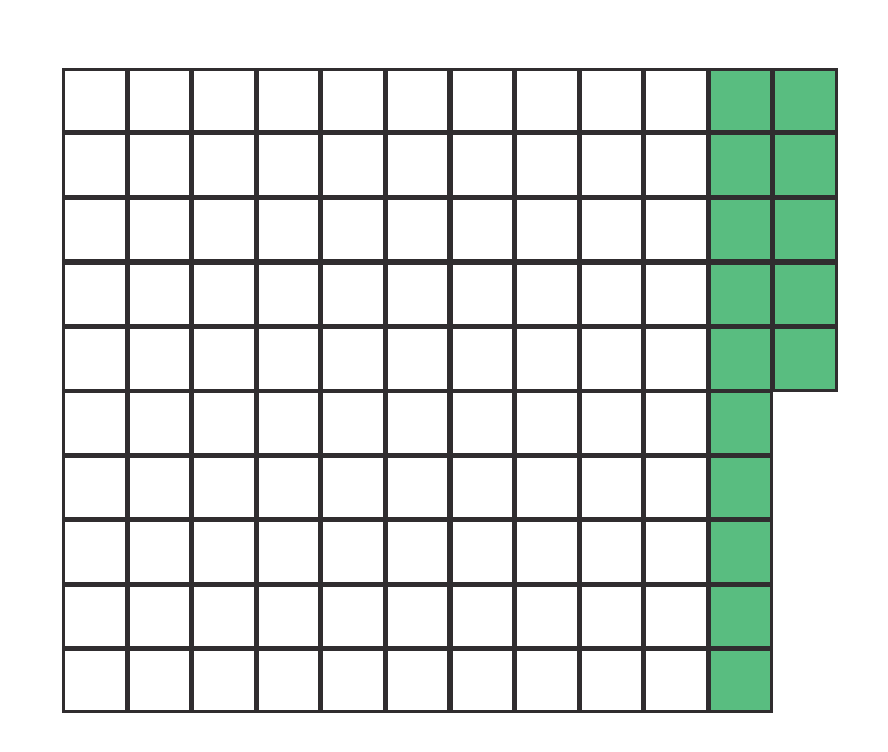
\includegraphics[scale=.25]{pictures/Kuva13-3-115.pdf}
    \end{center}
\end{esimerkki}

\begin{esimerkki}
Eräs kauppa myy tuotteitansa viiden prosentin alennuksella. Kuinka suuri on alennettu hinta, kun tuotteen tavallinen hinta on
\alakohdat{
§ $100$ euroa
§ $14,50$ euroa
}
	\begin{esimratk}
	\alakohdat{
§ Tämä tarkoittaa, että jokaisesta hinnasta vähennetään $\frac{5}{100}$ kertaa tuotteen hinta. $5\,\%$:n alennuksen osuus $100$ eurosta saadaan kertomalla $100$ euroa $5\,\%$:lla eli viidellä sadasosalla:
\[
\frac{5}{100} \cdot 100\,\text{euroa} = 5\,\text{euroa}
\]
Alennettu hinta saadaan vähentämällä alkuperäisestä hinnasta alennus eli $100\,\text{euroa} - 5\,\text{euroa} = 95\,\text{euroa}$.

§ Jos tuotteen alkuperäinen hinta on $14,50$ euroa, on alennuksen määrä
\[
	\frac{5}{100} \cdot 14,50\,\text{euroa} = 0,725\,\text{euroa}.
\]
Alennettu hinta on tällöin $(14,50 - 0,725)\,\text{euroa} \approx 13,78\,\text{euroa}$.

Samaan tulokseen pääsee vielä kätevämmin, kun ajattelee alennuksen määrän sijaan sitä, kuinka suuri osa hinnasta jää jäljelle. Jos alennus on $5\,\%$, jää hinnasta jäljelle $100\,\% - 5\,\% = 95\,\%$. Jos alkuperäinen hinta on $14,50$ euroa, on alennettu hinta 
\[
	\frac{95}{100} \cdot 14,50\,\text{euroa} \approx 13,78\,\text{euroa}.
\]
}
		\end{esimratk}
%		\begin{esimvast}
%		\alakohdat{
%		§
%		§
%		}
%		\end{esimvast}
\end{esimerkki}

\begin{esimerkki}
Tuotteen hintaa korotettiin $15$\,\%, jolloin hinnaksi muodostui $175$\,euroa. Kuinka suuri oli alkuperäinen korottamaton hinta?
	\begin{esimratk}
Olkoon alkuperäinen hinta $x$\,euroa. Koska hintaa on korotettu $15$\,\%, on uusi hinta $115$\,\% alkuperäisestä eli alkuperäinen hinta $x$ on kerrottu $1,15$:llä:
\begin{align*}
	1,15x	&= 175	&	&|\, \text{Jaetaan } 1,15\text{:llä}.\\
	x	&= \frac{175}{1,15} \approx 152,17
\end{align*}
	\end{esimratk}
    \begin{esimvast}
    Tuotteen alkuperäinen hinta oli $152,17$\,euroa.
    \end{esimvast}
\end{esimerkki}

%vastaava tehtävä: Sukkienhintaaalennettiin50%. Kuinka monta prosenttia hintaa täytyy nostaa, jotta saavutetaan alkuperäinen hinta?
%ja kuivausesimerkkejä...

\begin{esimerkki}
Elintarvikkeiden arvonlisävero alennettiin aikoinaan $17$\,\%:sta $12$\,\%:iin eli arvonlisäverokanta pieneni viidellä prosenttiyksiköllä. Muutoksen jälkeen muutamat nimeltä mainitsemattomat elintarvikeketjut mainostivat, että myyntihintoja oli laskettu keskimäärin $4,3$\,\%. Oliko arvonlisäveron alennus siirtynyt kokonaan hintoihin vai nostivatko kaupat katteitaan?
	\begin{esimratk}
	Merkitään mielivaltaista tuotteen verotonta hintaa $a$:lla. Koska arvonlisävero lisätään aina verottomaan hintaan, oli tuotteen verollinen hinta ennen $1,17a$ ja muutoksen jälkeen $1,12a$. Lasketaan, kuinka monta prosenttia verolliset hinnat laskivat, mikä tarkoittaa samaa kuin ''kuinka prosenttia uusi hinta on vanhaa pienempi'':
$$\frac{1,17a-1,12a}{1,17a}=\frac{0,05a}{1,17a}=\frac{0,05}{1,17}\approx 4,3\,\%$$

Myyntihintojen $4,3$ prosentin lasku selittyy siis käytännössä kokonaisuudessan arvonlisäveron laskulla. Tässä tapauksessa kukaan ei vetänyt välistä, vaan hinnat laskivat juuri kuin olisi odotettukin, jos vain veron osuus vähenee eikä verottomiin hintoihin kosketa.
	\end{esimratk}
\end{esimerkki}

Niin kuin prosenttiosuuksien laskemisessakin, useita prosentuaalisia muutoksia voidan ketjuttaa. On myös tärkeää huomata, että jos luvulle tehdään useita suhteellisia muutoksia, niiden järjestyksellä ei kertolaskun vaihdannaisuuden nojalla ole mitään väliä.

\begin{esimerkki}
Elokuvateatteri nosti lippujensa hintoja $20$\,\%. Taloustutkimuksiin tutustumisen jälkeen teatteri totesi halvemman hinnan tuovan enemmän asiakkaita, jolloin tulot kokonaisuudessaan kasvaisivat, joten lippujen hintoja laskettiin $25$\,\%.
\alakohdat{
§ Kuinka monta prosenttia lippujen hinnat lopulta muuttuivat alkuperäiseen nähden?
§ Entä jos olisi ensin laskettu hintoja $25$\,\% ja sitten korotettu samat $20$\,\%?
§ Jos lippujen hinta muutoksien jälkeen oli $7,00$ euroa, niin mikä oli niiden alkuperäinen hinta?
}
	\begin{esimratk}
	Merkataan tuntematonta lippujen hintaa esimerkiksi $x$:llä.
	\alakohdat{
	§ Hinnankorotuksen jälkeen lippujen hinta oli $1,20x$. Lippujen hinnan alentamisen jälkeen hinta on $0,75\cdot 1,20x$, eli $0,90x$. Hinnat olivat siis laskeneet yhteensä kymmenen prosenttia.
	§ Koska peräkkäiset suhteelliset muutokset lopulta formalisoituvat kertolaskuna ($0,75\cdot 1,20$), ja kertolasku on vaihdannainen, myös $1,20\cdot 0,75$ olisi tuottanut saman lopputuloksen. Hinnan muutosten järjestyksellä ei siis ole väliä.
	§ Edellisten kohtien perusteella saadaan yhtälö $0,90x=7,00\,€$, joka ratkeaa jakolaskulla, ja uudeksi hinnaksi saadaan $x=\frac{7,00\,€}{0,90\,€}\approx 7,78\,€$.
	}
	\end{esimratk}
\end{esimerkki}

\begin{esimerkki}
Ohut pilvipeite estää $10$\,\% auringon UV-säteilystä. Tiedetään myös, että varjossa oleskelu puolittaa saadun UV-annoksen. Kuinka monta prosenttia varjossa oleskelu pilvisellä säällä vähentää UV-annosta (verrattuna pilvettömään auringonottoon)?
	\begin{esimratk}
UV-säteilyn täydelle voimakkuudelle/määrälle/annokselle (säteilyn tyyppiä tai suuretta ylipäätään ei ole täsmennetty) ei tiedetä mitään lukuarvoa, joten merkitään sitä esimerkiksi $a$:lla. Koska pilvipeite estää $10$\,\% säteilystä, se päästää lävitseen $90$\,\%.  Pilvipeitteen läpäistyään säteilystä on siis jäljellä $90\,\%\cdot a=0,90a$. (Tämän voi laskea myös ''suoraan'' $a-0,10a=(1-0,10)a=0,90a$ ilman sanallista päättelyä läpipääsemisen ja estämisen yhteydestä.) Tämä lisäksi puolittuu (eli $50$\,\% pois) varjossa, eli lopulliseksi säteilymääräksi saadaan $0,50\cdot 0,90a$. Prosenttikertoimet voidaan yhdistää laskemalla kertolasku $0,50\cdot 0,90=0,45a$. Säteilystä on enää jäljellä siis vain $45$\,\%, joten pilvisyys ja varjoisuus on vähentänyt säteilyä $55\,\%$. (Tämän voisi näyttää laskuna ottamalla jäljellä oleva osuus $0,45a$ pois alkuperäisestä $a$:sta: $a-0,45a=(1-0,45)a=0,55a$.)
	\end{esimratk}
	\begin{esimvast}
	$55$ prosenttia
	\end{esimvast}
\end{esimerkki}

\begin{esimerkki}
Osoitetaan, että jos mielivaltainen nollasta poikkeava luku $y$ kasvaa ensin $p$ prosenttia ($p>0$) ja sen jälkeen pienee samat $p$ prosenttia, emme päädy takaisin alkuperäiseen lukuun $y$. $p$ prosentin kasvu antaa prosenttikertoimen $(1+\frac{p}{100})$, ja $p$:llä pienentäminen antaa prosenttikertoimen $(1-\frac{p}{100})$. Kun edellä mainitut yhdistetään, saadaan muutosten jälkeiseksi luvuksi $(1-\frac{p}{100})(1+\frac{p}{100})y$. Koska tekijä $y$ on alkuperäinen perusarvo, riittää osoittaa, että prosenttikerroin ei voi saada arvoa $1$. Jos se voisi saada arvon $1$, niin olisi mahdollista päätyä takaisin perusarvoon. Sievennetään prosenttikertoimen lauseketta:
\begin{align*}
&(1-\frac{p}{100})(1+\frac{p}{100}) && || \text{sovelletaan osittelulakia (puretaan oikeanpuoleiset sulkeet)} \\
&=(1-\frac{p}{100})\cdot 1 + (1-\frac{p}{100})\cdot \frac{p}{100} && || \text{yhdellä kertominen} \\
&=1-\frac{p}{100} + (1-\frac{p}{100})\cdot \frac{p}{100} && || \text{sovelletaan osittelulakia (avataan oikeanpuoleiset sulkeet)} \\
&=1-\frac{p}{100} + 1\cdot \frac{p}{100}-\frac{p}{100}\cdot \frac{p}{100}  && || \text{yhdellä kertominen ja oikeanpuoleinen kertolasku} \\
&=1-\frac{p}{100} + \frac{p}{100}-\frac{p^2}{10\,000}  && || \text{erimerkkiset termit kumoutuvat} \\
&=1-\frac{p^2}{10\,000}  && \\
\end{align*}
Murtolauseke $\frac{p^2}{10\,000}$ saa arvon nolla, jos ja vain jos sen osoittaja $p^2$ saa arvon nolla. Koska lähtöoletus oli, että prosentuaalinen muutos on nollasta poikkeava, ei $p^2$ voi olla nolla. Niin myöskään erotuksesta $1-\frac{p^2}{10\,000}$ ei voi tulla tasan yhtä, eikä prosenttikerron näin voi saada tasan arvoa $1$. Siis $p$ prosentilla kasvattaminen ja sen jälkeen pienentäminen ei voi tuottaa uudelleen alkuperäistä arvoa (kunhan alkuperäinen arvo tai prosentuaalinen muutos eivät ole nollia).
\end{esimerkki}

%Jos sama suhteellinen muutos toistuu useita kertoja, lauseke sievenee potenssin avulla. +esim.

Jos jokin käsiteltävä kaava koostuu muuttujien tulosta, voidaan siihen suoraan sijoittaa yksittäisten muuttujien suhteelliset muutokset prosenttikertoimien avulla. Erilliset prosenttikertoimet voidaan kaikki siirtää alkuperäisen lausekkeen eteen, yhdistää ja tulkita siitä kokonaisvaikutus.

\begin{esimerkki}
%\alakohdat{
%§
Jos kuution särmän pituus on $a$, niin kuution tilavuus on $a^3$. Jos jokaista särmää pidennetään viisi prosenttia, niin miten kuution tilavuus muuttuu?
%§ Hakkuupuuta mallinnetaan suorana ympyräkartiona, jonka tilavuus voidaan laskea kaavalla $V=\frac{1}{3}\pi r^2h$, missä $r$ on säde eli halkaisijan puolikas pohjan tasolla, ja $h$ on puun korkeus. Kuinka paljon puun tilavuus on kasvanut, kun vuoden kuluttua mittauksissa todetaan puun paksuuntuneen neljä prosenttia ja kasvaneen pituutta kymmenen prosenttia?
%}
	\begin{esimratk}
	%\alakohdat{
%§
$V=a^3$ on alkuperäinen tilavuus. Korvataan nyt (jokainen) $a$ kasvaneella versiolla $1,05a$, jolloin saadaan lauseke $(1,05a)^3$. Tästä saadaan tulon potenssina $1,05^3a^3 \approx 1,158a^3$. Vertaamalla alkuperäiseen tilavuuteen $a^3$ todetaan, että tilavuus on kasvanut noin $15,8$ prosenttia. %tarkista vastaustarkkuus
%§
%}
	\end{esimratk}
\end{esimerkki} %merkitsevät numerot prosenttilaskuissa!!!

Jos tehtävässä käsitellään useita suureita, ole tarkkana, että muutos kohdistetaan oikeaan suureeseen. Esimerkiksi työnteosta tai matkustamisesta puhuttaessa saatetaan arkisesti sanoa ''nopeammin'', vaikka tarkoitetaan oikeasti \textit{lyhyempää kestoa}. Nopeampi suoritus toki johtaa lyhyempään kestoon, mutta suhteelliset muutokset eivät ole lukuarvoltaan samat.

\begin{esimerkki}
Junakantaa uusitaan, ja uudet junat ovat $15$ prosenttia nopeammin kuin vanhat. Kuinka monta prosenttia matkojen kestot lyhenevät? Pyöritellen kaavaa $v=\frac{s}{t}$, missä $v$ on (keski)nopeus, $s$ on matkan pituus ja $t$ on matkaan kuluva aika, saadaan matkan kestoksi ratkaistua $t=\frac{s}{v}$. Korvataan nyt entinen nopeus $v$ uudella nopeudella $1,15v$, jolloin uudeksi matkan kestoksi saadaan $\frac{s}{1,15v}=\frac{1}{1,15}\frac{s}{v}=\frac{1}{1,15}t$. Prosenttikertoimen $\frac{1}{1,15}$ likiarvo on $0,87$, eli uusi matkan kesto on $0,87t$. Kertoimesta nähdään, että matkan kesto lyheni $13$ prosentilla, eikä siis $15$ prosentilla, niin kuin nopeus muuttui!
\end{esimerkki}

%laske esimerkkinä yhteys kahden sovellustyypin välille. a-> 1,34a & (1,34a-a)/a)=0,34
%yo-tehtävälistaan se lyhyen matikan järjestystehtävä